\documentclass[a4paper]{article}\usepackage[]{graphicx}\usepackage[]{color}
%% maxwidth is the original width if it is less than linewidth
%% otherwise use linewidth (to make sure the graphics do not exceed the margin)
\makeatletter
\def\maxwidth{ %
  \ifdim\Gin@nat@width>\linewidth
    \linewidth
  \else
    \Gin@nat@width
  \fi
}
\makeatother

\definecolor{fgcolor}{rgb}{0.345, 0.345, 0.345}
\newcommand{\hlnum}[1]{\textcolor[rgb]{0.686,0.059,0.569}{#1}}%
\newcommand{\hlstr}[1]{\textcolor[rgb]{0.192,0.494,0.8}{#1}}%
\newcommand{\hlcom}[1]{\textcolor[rgb]{0.678,0.584,0.686}{\textit{#1}}}%
\newcommand{\hlopt}[1]{\textcolor[rgb]{0,0,0}{#1}}%
\newcommand{\hlstd}[1]{\textcolor[rgb]{0.345,0.345,0.345}{#1}}%
\newcommand{\hlkwa}[1]{\textcolor[rgb]{0.161,0.373,0.58}{\textbf{#1}}}%
\newcommand{\hlkwb}[1]{\textcolor[rgb]{0.69,0.353,0.396}{#1}}%
\newcommand{\hlkwc}[1]{\textcolor[rgb]{0.333,0.667,0.333}{#1}}%
\newcommand{\hlkwd}[1]{\textcolor[rgb]{0.737,0.353,0.396}{\textbf{#1}}}%
\let\hlipl\hlkwb

\usepackage{framed}
\makeatletter
\newenvironment{kframe}{%
 \def\at@end@of@kframe{}%
 \ifinner\ifhmode%
  \def\at@end@of@kframe{\end{minipage}}%
  \begin{minipage}{\columnwidth}%
 \fi\fi%
 \def\FrameCommand##1{\hskip\@totalleftmargin \hskip-\fboxsep
 \colorbox{shadecolor}{##1}\hskip-\fboxsep
     % There is no \\@totalrightmargin, so:
     \hskip-\linewidth \hskip-\@totalleftmargin \hskip\columnwidth}%
 \MakeFramed {\advance\hsize-\width
   \@totalleftmargin\z@ \linewidth\hsize
   \@setminipage}}%
 {\par\unskip\endMakeFramed%
 \at@end@of@kframe}
\makeatother

\definecolor{shadecolor}{rgb}{.97, .97, .97}
\definecolor{messagecolor}{rgb}{0, 0, 0}
\definecolor{warningcolor}{rgb}{1, 0, 1}
\definecolor{errorcolor}{rgb}{1, 0, 0}
\newenvironment{knitrout}{}{} % an empty environment to be redefined in TeX

\usepackage{alltt}
\usepackage{a4wide}
\usepackage[margin=.8in]{geometry}
\usepackage{colortbl}

\title{Comparison of Versions of Kinship Links}
\author{Joe Rodger's BG Team}
\IfFileExists{upquote.sty}{\usepackage{upquote}}{}
\begin{document}

\maketitle

\definecolor{goodColor}{rgb}{.9,1,.85}
\definecolor{sosoColor}{rgb}{1,0.9215686,0.6117647}
\definecolor{badColor}{rgb}{1,.85,.85}
\definecolor{nullColor}{rgb}{.9, 0.85, 0.95} %0.8000000 0.7529412 0.8549020
\setlength{\parindent}{0pt}%http://tex.stackexchange.com/questions/49188/how-to-insert-vertical-space-between-paragraphs

% Working directory: getwd();



% Working directory: getwd();












\begin{knitrout}
\definecolor{shadecolor}{rgb}{0.969, 0.969, 0.969}\color{fgcolor}\begin{kframe}
\begin{verbatim}
##              DBMS_Name               DBMS_Ver        Driver_ODBC_Ver       Data_Source_Name 
## "Microsoft SQL Server"           "13.00.4206"                "03.80"     "local-nlsy-links" 
##            Driver_Name             Driver_Ver               ODBC_Ver            Server_Name 
##      "msodbcsql13.dll"           "14.00.0500"           "03.80.0000" "GIMBLE\\EXPRESS_2016"
## Time difference of 0.8384829 secs
## [1] 22176
\end{verbatim}
\end{kframe}
\end{knitrout}



% \textbf{RelationshipPaths Considered}: includedRelationshipPaths;\\
\textbf{Newer Links Version}: 85;
\textbf{Older Links Version}: 84;




\begin{knitrout}
\definecolor{shadecolor}{rgb}{0.969, 0.969, 0.969}\color{fgcolor}\begin{kframe}
\begin{verbatim}
Newer Links: R excludes 0, .0625, .125 (as well as .375 & .75)
Older Links: Adds Gen1 back
\end{verbatim}
\end{kframe}
\end{knitrout}

\begin{figure}[htbp]
\begin{knitrout}
\definecolor{shadecolor}{rgb}{0.969, 0.969, 0.969}\color{fgcolor}
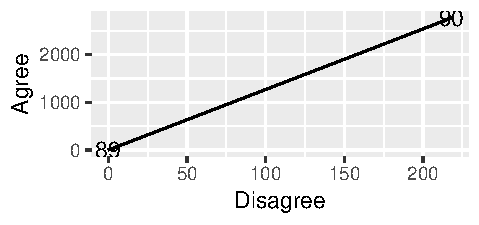
\includegraphics[width=\maxwidth]{figure/unnamed-chunk-2-1} 

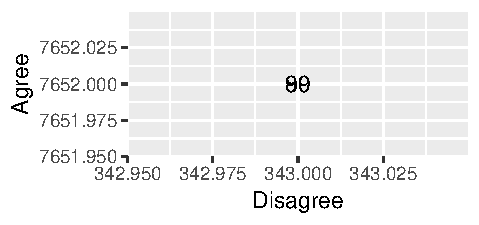
\includegraphics[width=\maxwidth]{figure/unnamed-chunk-2-2} 

\end{knitrout}
\caption{ROC for Gen1Housemates (left) and Gen2Siblings (right)}
\end{figure}

% latex table generated in R 3.4.1 by xtable 1.8-2 package
% Thu Sep 14 17:11:54 2017
\begin{table}[ht]
\centering
\begingroup\large
\begin{tabular}{lrrrrr}
  \hline
R & Implicit2004 & Implicit & Roster & Explicit & Eventual \\ 
  \hline
- &   0 &   0 &   0 &   0 &   0 \\ 
   \hline
\end{tabular}
\endgroup
\caption{Counts for Gen1Housemates} 
\end{table}
% latex table generated in R 3.4.1 by xtable 1.8-2 package
% Thu Sep 14 17:11:54 2017
\begin{table}[ht]
\centering
\begingroup\large
\begin{tabular}{lrrrrr}
  \hline
R & Implicit2004 & Implicit & Roster & Explicit & Eventual \\ 
  \hline
- &   0 &   0 &   0 &   0 &   0 \\ 
   \hline
\end{tabular}
\endgroup
\caption{Counts for Gen1Housemates (Previous version of links)} 
\end{table}
% latex table generated in R 3.4.1 by xtable 1.8-2 package
% Thu Sep 14 17:11:54 2017
\begin{table}[ht]
\centering
\begingroup\large
\begin{tabular}{lrrrr}
  \hline
R & Implicit2004 & Implicit & Explicit & Eventual \\ 
  \hline
0.25 & 2221 & 3012 & 2975 & 3442 \\ 
  0.375 & 2663 & - & 244 & 610 \\ 
  0.5 & 5778 & 6731 & 5599 & 6997 \\ 
  0.75 & - &  12 & - &  12 \\ 
  1 &  36 &  27 &  22 &  27 \\ 
  - & 390 & 1306 & 2248 &   0 \\ 
   \hline
\end{tabular}
\endgroup
\caption{Counts for Gen2Siblings} 
\end{table}
% latex table generated in R 3.4.1 by xtable 1.8-2 package
% Thu Sep 14 17:11:54 2017
\begin{table}[ht]
\centering
\begingroup\large
\begin{tabular}{lrrrr}
  \hline
R & Implicit2004 & Implicit & Explicit & Eventual \\ 
  \hline
0.25 & 2221 & 3012 & 2975 & 3442 \\ 
  0.375 & 2663 & - & 244 & 610 \\ 
  0.5 & 5778 & 6731 & 5599 & 6997 \\ 
  0.75 & - &  12 & - &  12 \\ 
  1 &  36 &  27 &  22 &  27 \\ 
  - & 390 & 1306 & 2248 &   0 \\ 
   \hline
\end{tabular}
\endgroup
\caption{Counts for Gen2Siblings (Previous version of links)} 
\end{table}


% latex table generated in R 3.4.1 by xtable 1.8-2 package
% Thu Sep 14 17:11:54 2017
\begin{table}[ht]
\centering
\begin{tabular}{rrrrlr}
  \hline
Count & RImplicit2004 & RImplicit & RExplicit & RRoster & Delta \\ 
  \rowcolor{goodColor}  \hline
4406 & 0.500 & 0.500 & 0.500 & - & 0 \\ 
   \rowcolor{goodColor} 1599 & 0.250 & 0.250 & 0.250 & - & 0 \\ 
  1095 & 0.500 & 0.500 & - & - & 0 \\ 
   \rowcolor{goodColor} 534 & 0.375 & 0.500 & 0.500 & - & 0 \\ 
   \rowcolor{goodColor} 532 & 0.375 & 0.250 & 0.250 & - & 0 \\ 
   \rowcolor{nullColor} 478 & 0.375 & - & - & - & 0 \\ 
   \rowcolor{sosoColor} 369 & 0.375 & - & 0.250 & - & 0 \\ 
   \rowcolor{sosoColor} 257 & 0.375 & - & 0.500 & - & 0 \\ 
  208 & 0.250 & 0.250 & - & - & 0 \\ 
  169 & 0.375 & 0.500 & - & - & 0 \\ 
  121 & 0.375 & 0.250 & - & - & 0 \\ 
   \rowcolor{goodColor} 119 & - & 0.500 & 0.500 & - & 0 \\ 
   \rowcolor{goodColor} 109 & 0.500 & 0.250 & 0.250 & - & 0 \\ 
   \rowcolor{goodColor} 98 & - & 0.250 & 0.250 & - & 0 \\ 
  91 & 0.250 & 0.250 & 0.375 & - & 0 \\ 
   \rowcolor{badColor} 86 & 0.250 & 0.250 & 0.500 & - & 0 \\ 
   \rowcolor{badColor} 77 & 0.375 & 0.250 & 0.500 & - & 0 \\ 
   \rowcolor{badColor} 75 & 0.500 & 0.500 & 0.250 & - & 0 \\ 
  75 & - & 0.500 & - & - & 0 \\ 
   \rowcolor{goodColor} 73 & 0.250 & 0.500 & 0.500 & - & 0 \\ 
   \rowcolor{sosoColor} 66 & 0.250 & - & 0.250 & - & 0 \\ 
   \rowcolor{badColor} 50 & 0.375 & 0.500 & 0.250 & - & 0 \\ 
   \rowcolor{badColor} 41 & 0.250 & 0.500 & 0.250 & - & 0 \\ 
  41 & 0.500 & 0.500 & 0.375 & - & 0 \\ 
   \rowcolor{sosoColor} 30 & 0.375 & - & 0.375 & - & 0 \\ 
   \rowcolor{sosoColor} 29 & - & - & 0.250 & - & 0 \\ 
   \rowcolor{nullColor} 29 & - & - & - & - & 0 \\ 
  23 & 0.375 & 0.250 & 0.375 & - & 0 \\ 
  23 & 0.375 & 0.500 & 0.375 & - & 0 \\ 
   \rowcolor{goodColor} 21 & 1.000 & 1.000 & 1.000 & - & 0 \\ 
   \rowcolor{badColor} 18 & 0.500 & 0.250 & 0.500 & - & 0 \\ 
   \rowcolor{sosoColor} 17 & 0.250 & - & 0.500 & - & 0 \\ 
  17 & - & 0.250 & - & - & 0 \\ 
  15 & 0.500 & 0.250 & 0.375 & - & 0 \\ 
   \rowcolor{nullColor} 14 & 0.250 & - & - & - & 0 \\ 
  13 & 0.250 & 0.500 & - & - & 0 \\ 
  12 & 1.000 & 0.750 & - & - & 0 \\ 
  11 & 0.500 & 0.250 & - & - & 0 \\ 
  10 & 0.250 & 0.500 & 0.375 & - & 0 \\ 
   \rowcolor{sosoColor} 6 & - & - & 0.500 & - & 0 \\ 
   \rowcolor{badColor} 4 & - & 0.250 & 0.500 & - & 0 \\ 
   \rowcolor{badColor} 4 & - & 0.500 & 0.250 & - & 0 \\ 
   \rowcolor{sosoColor} 3 & 0.250 & - & 0.375 & - & 0 \\ 
   \rowcolor{sosoColor} 3 & 0.500 & - & 0.250 & - & 0 \\ 
  3 & 1.000 & 1.000 & - & - & 0 \\ 
  3 & - & 0.250 & 0.375 & - & 0 \\ 
  3 & - & 0.500 & 0.375 & - & 0 \\ 
   \rowcolor{sosoColor} 2 & 0.500 & - & 0.500 & - & 0 \\ 
   \rowcolor{sosoColor} 2 & - & - & 0.375 & - & 0 \\ 
   \rowcolor{goodColor} 1 & 0.500 & 1.000 & 1.000 & - & 0 \\ 
  1 & 0.500 & 1.000 & - & - & 0 \\ 
   \rowcolor{nullColor} 1 & 0.500 & - & - & - & 0 \\ 
  1 & - & 1.000 & - & - & 0 \\ 
   \hline
\end{tabular}
\caption{Counts for Gen2Siblings} 
\end{table}



\end{document}
